\documentclass[conference]{IEEEtran}
\IEEEoverridecommandlockouts
% The preceding line is only needed to identify funding in the first footnote. If that is unneeded, please comment it out.
\usepackage{cite}
\usepackage{amsmath,amssymb,amsfonts}
\usepackage{algorithmic}
\usepackage{graphicx}
\usepackage{textcomp}
\usepackage{xcolor}
\usepackage{booktabs}
\usepackage{placeins}
\def\BibTeX{{\rm B\kern-.05em{\sc i\kern-.025em b}\kern-.08em
    T\kern-.1667em\lower.7ex\hbox{E}\kern-.125emX}}
\begin{document}

\title{Rangefinder-Calibrated Monocular Depth Estimation}

\author{
	\IEEEauthorblockN{Raj Anadkat}
	\IEEEauthorblockA{raj618@seas.upenn.edu}
\and
	\IEEEauthorblockN{Jonathan Lee}
	\IEEEauthorblockA{jonlee27@seas.upenn.edu}
\and
	\IEEEauthorblockN{Jonathan Schoeffling}
	\IEEEauthorblockA{jschoeff@seas.upenn.edu}
\and
	\IEEEauthorblockN{Hanli Zhang}
	\IEEEauthorblockA{hanlizh@seas.upenn.edu}
}

\maketitle

\begin{abstract}
The lidar used on the F1TENTH platform is expensive, which limits the size of
the classes and programs that use it. This project aimed to achieve a more
useful combined estimate of both azimuth and range by fusing data from high
azimuth accuracy / low range accuracy sensors with data from low azimuth
accuracy / high range accuracy accuracy sensors. Additional work is needed to
overcome noise in the depth estimation model and to reliably associate the
measurements of each sensor.
\end{abstract}

\begin{IEEEkeywords}
F1TENTH, autonomous driving, MiDaS, time-of-flight, rangefinder, lidar, sensor
fusion
\end{IEEEkeywords}

\section{Project Objectives}
To function as an autonomous vehicle, the F1TENTH platform must be able to
determine the location of objects in its environment, with a reasonable degree
of accuracy in both azimuth and range. The lidars currently used for this task
are the single most expensive component on the car. An alternate solution that
can achieve reasonable accuracy with lower cost would be of substantial
benefit.

MiDaS is a machine learning model capable of vision-based depth inference.
Using a monocular camera as an input, the model can produce outputs with high
accuracy in azimuth and elevation, but its output is a low-fidelity estimate of
inverse relative depth. Laser time-of-flight sensors, by contrast, have
excellent accuracy in depth, but can only provide azimuth information in a
fixed angle increments with a fairly wide field of view. The objective of the
project is to use sensor fusion to combine the high-accuracy azimuth and
elevation data from MiDaS with the high-accuracy range data from an array of
time-of-flight sensors, leveraging the strengths of both sensors to produce a
fused depth map with reasonable accuracy in all dimensions.


\section{Implementation}

\subsection{System Design}

The design physically mounts a camera above an array of rangefinders, with each
sensor element in the array spaced in even increments of angle so that coverage
is provided for the entire field of view of the RealSense camera. The mount is
shown in Figure \ref{fig:mount}.

\begin{figure}
\centering
\includegraphics[scale=1.00]{mount.png}
\caption{Sensor array mount attached to the F1TENTH car}
\label{fig:mount}
\end{figure}


\begin{figure}
\centering
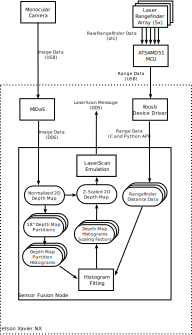
\includegraphics[scale=0.31]{block-diagram-final.png}
\caption{Block diagram for the sensor system}
\label{fig:block-diagram}
\end{figure}


The Intel RealSense camera, operating in this configuration as a monocular
camera, provides inputs to the MiDaS depth estimation model. The output of the
model is a 960x540 grayscale image, providing the model's 2D estimation of
inverse relative depth. Concurrently, each element of the time-of-flight sensor
array samples distances within its field of view, and provides them to the
Jetson via USB.

A sensor fusion node running on the Jetson receives both the depth map and the
direct range measurments, which are then combined to produce an absolute depth
map. This absolute depth map is then sampled at a predetermined height, and the
range values are packed into a ROS LaserScan message, which emulates the output
of the lidar. The follow-the-gap algorithm then consumes this message to steer
the car.

The overall sensor design is shown in Figure \ref{fig:block-diagram}.

\FloatBarrier

\subsection{Monocular Depth Estimation}
Monocular depth estimation is a task of predicting the depth map of a given input image. This can be formulated as a pixel-wise regression problem where each pixel in the input image is assigned a depth value. The task can be viewed as a segmentation problem where each pixel is considered a class and predicted depth is assigned to that class. The predicted depth maps can be used for various applications such as 3D reconstruction and mapping.

There are various state-of-the-art models available for monocular depth estimation. Early models such as single-image depth prediction (SID) and depth from a single image (DFSI) used traditional computer vision techniques such as edge detection and texture analysis. Recently, deep learning-based models have shown promising results for monocular depth estimation. These models can be categorized into two groups: (1) Direct regression-based models, such as Fully Convolutional Networks (FCNs) and Deep Depth Regression (DDR), which directly estimate the depth from an image; and (2) Indirect methods, such as Monocular Depth Estimation via Semantic Transfer (MiDaS) and Depth from a Focus Stack (DFF), which predict the depth indirectly by leveraging the relationship between depth and other visual cues such as semantic information or focus cues.

The team initially attempted to develop a custom monocular depth estimation model utilizing the Unet architecture with a 256x256x3 input size to predict depth maps. The model comprised upscaling and downscaling blocks, with the objective of optimizing three losses: SSIM loss, L1 loss, and depth smoothness loss. The model was trained on the NYU V2 Dataset. However, the model yielded unsatisfactory results, prompting the team to enhance the model by replacing the encoding part of the Unet model with a pretrained DenseNet-201 backbone.

The team adopted a similar model, which exhibited remarkable performance. The Unet model with DenseNet-201 backbone achieved superior performance, with a 640x480 input size capable of capturing larger depths. Nevertheless, after TensorRT optimization, the inference speed was only 4 fps, thereby prompting the team to switch to the MiDaS v21 small 256 model due to its moderate accuracy, lightweight, and efficient nature. The table presented below illustrates the depth maps generated by three different models, along with their corresponding input size, inference speed on Jetson, and depth maps.

\begin{table}[htbp]
\centering
\caption{Depth map comparison for the three models.}
\label{tab:model_comparison}
\small % smaller font size
\begin{tabular}{|p{1.4cm}|p{1.2cm}|p{1cm}| p{2.5cm}|}
\hline
\textbf{Model} & \textbf{Input} & \textbf{FPS} & \textbf{Depth Map} \\
\hline
Custom UNet & 256x256 & N/A &  \includegraphics[width=1\linewidth]{custom_Unet.png} \\ \hline
DenseNet-201 & 640x480 & 4  & \includegraphics[width=1\linewidth]{densenet.png} \\ \hline
MiDaS v21 Small & 256x256 & 40  & \includegraphics[width=1\linewidth]{midas.png} \\ \hline
\end{tabular}
\end{table}


The outputs generated by the monocular depth estimation model are relative inverse depths. In order to retrieve absolute depths for each frame, we need to obtain at least two pixels with model outputs and ground truth depths to calculate a scaling factor and a bias. This process can be facilitated through the use of time-of-flight sensors and the approach outlined in the subsequent sections.
\FloatBarrier
\subsection{Time-of-Fight Array}
The time-of-flight sensor array is composed of five of ST Microelectronics'
VL53L4CX sensors, mounted to the corresponding Adafruit breakout board. The
sensors connect via I2C to an Adafruit Metro M4 Grand Central development
board, hosting an ATSAMD51 microcontroller, which performs the requisite signal
processing and then provides the range data to the host via USB. A client
library implementing a libusb device driver provides access to the rangefinder
data.

\begin{figure}
\centering
\includegraphics[scale=0.31]{vl53l4cx-adafruit.png}
\caption{the VL53L4CX time-of-flight sensor on Adafruit breakout board}
\label{fig:vl53l4cx}
\end{figure}

\begin{figure}
\centering
\includegraphics[scale=0.31]{grand-central.png}
\caption{the Adafruit Metro M4 Grand Central development board}
\label{fig:grand-central}
\end{figure}

The the physical mount is shown in \ref{fig:mount}. It is 3D printed from ABS
plastic and serves as an attachment point for both the laser rangefinders and
the Intel RealSense camera. The mount is split into two halves. The lower mount
show in the left side of Figure \ref{fig:split-mount} attaches to the v3
version of the F1TENTH upper chassis, in place of the Hokuyo Lidar, and also
provides screwholes to attach the SAMD51 development board.

The upper mount attaches to the lower mount with screws, and provides the
attachment points for the camera and rangefinders. The camera and rangefinders
are positioned such that the camera lens is approximately at the center of a
circle with the time of flight sensors along the circumference. The sensors are
positioned such that their 18-degree fields of view are adjacent and provide
full coverage over the RealSense camera's 87-degree horizontal FOV. Because one
dimensions of each measurement is almost completely unknown to the other type
of sensor, using a mechanically aligned sensor configuration is preferred to
coordinate transformations.

\begin{figure}
\centering
\includegraphics[scale=0.20]{split-mount.png}
\caption{the lower and upper mount of the sensor array}
\label{fig:split-mount}
\end{figure}

Each of the 5 sensors is electrically connected over a single I2C bus. Power is
provided by the 3V3 power pin of the development board. With each sensor
drawing approximately 20mA of current, the total power consumption of 100mA is
low enough that the rangefinder array can be bus powered, eliminating the need
for an external power supply. Pinouts and cable drawings are shown in Figure
\ref{fig:cable-drawings}. The need to cable the I2C interfaces unfortunately
proved to be problematic while integrating with the F1TENTH car (see the
\textit{Results} section for details).

\begin{figure}
\centering
\includegraphics[scale=0.11]{cables/laser-array-cables.png}
\caption{cable drawings for the laser array}
\label{fig:cable-drawings}
\end{figure}

The SAMD51 microcontroller handles the I2C communications with the sensors,
initial signal processing, and communication with the host via USB. The I2C
protocol and signal processing for the sensor modules is handled by ST's VL53LX
library. A custom USB driver handles communications with the host. The USB
interface provides control transfers to manage the array, allowing each sensor
element to be independently enable/disabled. Interrupt transfers are used to
provide data on an 11-ms periodic.

\FloatBarrier

On the client side, the device driver was implemented in userspace using
libusb. This avoids the need for a kernel driver, improving portability. The
driver takes the form of C library with Python API bindings provided using
the ctypes foreign function interface.

\subsection{Sensor Fusion}
Sensor fusion is a critical component, enabling the integration and combination of data from multiple sensors to obtain a more accurate and reliable understanding of the environment. In our project, we employed sensor fusion techniques to combine depth information from a depth map and range measurements from a rangefinder. This fusion process aimed to enhance the accuracy and robustness of the depth estimation.

1) Depth Map Histogram Analysis:
One aspect of our sensor fusion approach involved analyzing the histogram of the depth map. The depth map represents the estimated depth values for each pixel in the image, and we sliced the depth map into different parts to align its view with the view of the TOF (Time-of-Flight) sensors. 


\begin{figure}[htbp]
    \centering
    \includegraphics[width=0.4\textwidth]{histogram_analysis.png}
    \caption{Histogram Analysis}
    \label{fig:Histogram Analysis}
\end{figure}

The histogram analysis allowed us to identify intensity peaks in the depth map. By extracting these intensity peaks, we could understand the presence of various objects and their approximate distances from the sensor.


2) Linear Regression for Scaling Factors and Biases:
To align the intensity peaks in the depth map histogram with the range measurements from the rangefinder, we utilized a linear regression algorithm. This algorithm produced scaling factors and biases that helped adjust the estimated depth values from the depth map to be more accurate and aligned with the range measurements.
The inverse depth values from the depth map and rangefinder can be represented as $z_{d} = 1/D$ and $z_{r} = 1/R$, respectively, where $D$ and $R$ represent the depth and range values. The linear regression approach involved finding the linear relationship between the absolute inverse depth values obtained from the rangefinder and the inverse depth values from the depth map. We can represent this relationship as:
$z_r=\alpha z_d+\beta$

where $\alpha$ and $\beta$ represent the scaling factor and bias, respectively. By deriving the scaling factors and biases, we could convert the relative inverse depth predictions from the depth map into absolute inverse depth values, enhancing the accuracy of the depth estimation.

3) Kalman Filter for Sensor Fusion:
In addition to the linear regression-based adjustment, we employed a sensor fusion algorithm known as the Kalman filter. 

The Kalman filter played a crucial role in integrating the adjusted depth values from the depth map with the range measurements from the rangefinder. By considering the respective strengths and weaknesses of the two sensors, the Kalman filter dynamically updated the scale and bias parameters, incorporating new information and refining the depth estimation.

Through the fusion process, the Kalman filter effectively combined the adjusted depth values and the range measurements, exploiting their complementary characteristics to provide a more accurate and reliable estimate of the scene's depth information.

\subsection{Gap Following}
TODO

\section{Results}
\subsection{Integrated Gap Following}
TODO

\subsection{MiDaS Performance}
The MiDAS depth estimation model performed decently on the levine corridors. With an impressive speed of 40 frames per second, it could efficiently generate depth maps in real-time after TensorRT optimization. Furthermore, the model's performance in terms of providing accurate depth information is commendable, making it a valuable asset in various applications that require depth estimation. However, it is important to note that the model is not immune to certain limitations, such as the presence of noise and susceptibility to reflections and optical illusions, as well as its training on non-consecutive images that may cause temporal inconsistency in video applications.It is worth mentioning that the MiDaS model tends to be biased towards hands and faces and may perceive their depths differently than other objects present at the same depths. To account for these problems, Transfer learning on depth maps from consecutive frames of Race Map Data-set can show promising results in reducing bias towards specific objects, reduce the temporal inconsistency and improve the overall performance of the model.  Despite these limitations, the MiDaS model remains a powerful solution for depth estimation tasks.

\subsection{Time-of-Fight Array Performance}
The outputs provided by the VL53L4CX time of flight sensors are unfortunately
somewhat less "rich" than originally hoped. Even after some tuning, the
rangefinders were only capable of measuring a maximum range of approximately
3.5 meters, as opposed to the advertised 6 meters. The tunable parameters
unfortunately have a tradeoff between maximum range and latency, both of which
are important for this application. Additionally, the "histogram" nature of the
rangefinder (i.e., being capable of detecting sensor returns at multiple
distances within its field of view) is somewhat less impressive in practice.
While five or six simultaneous returns have been seen under ideal
circumstances, this is uncommon, and typically, only a single value is
returned. This sharply limits the amount of data that can be used during the
sensor fusion regression step.

Another complication arises from integration with the F1TENTH car, which
appears to induce failures in the sensor's I2C communications. Each time the
motor is activated, the I2C bus fails, entering an inconsistent state shortly
thereafter. Diagnostics performed thus far have ruled out power transients and
mechanical shock and vibration as possible causes. The problem persists even
when the sensor is connected to an independent electrical system and data is
sent to an off-car USB host. Given the evidence, an EMI problem caused by
operating a large motor in close physical proximity to the sensor seems likely.
The use of separate development and breakout boards necessitates cables of
several centimeters in length to connect the I2C clock and data lines between
components. Unshielded cables of this length could very well form an antenna
that is susceptible to radiated emissions from the large inductive load of the
motor. This complication unfortunately limited the degree to which the sensor
fusion implementation could be evaluated operationally.

\subsection{Sensor Fusion Performance}
While our sensor fusion approach has shown promising results in combining depth information from the depth map and range measurements from the rangefinder, we have observed some limitations in the current implementation. Specifically, the sensor fusion outputs exhibit a certain level of inconsistency and fluctuations, resulting in a "jumpy" behavior.

One of the challenges we encountered is the need for more integration time to refine the implementation. The current fusion process combines the depth map and range measurements to obtain depth estimates, but the results still lack the desired smoothness and stability. This is mainly due to the inherent noise and uncertainty present in both the depth map and rangefinder data.

To address this issue and achieve more reliable and accurate depth estimation, additional refinement is required. Increasing the integration time, which involves collecting data over a longer period, can help mitigate the effects of noise and fluctuations. This extended integration time allows the sensor fusion algorithm to gather more information and make more informed decisions, resulting in smoother and more consistent depth outputs.

Furthermore, optimization of the sensor fusion algorithm itself may be necessary. Fine-tuning the fusion parameters, adjusting the weighting of the depth map and rangefinder data, and incorporating filtering techniques can contribute to improved performance. Techniques such as temporal filtering or applying smoothing algorithms, such as moving average or Gaussian filters, can help reduce the "jumpy" behavior and provide more stable depth estimates.

In conclusion, while our sensor fusion approach shows promise in combining depth information from the depth map and range measurements, there is room for improvement. 

\section{Future Work}
The existing model for monocular depth estimation can be further improved. Transfer learning approaches can be adopted on a custom dataset consisting of consecutive frames. This can help to mitigate the issue of temporal inconsistency and enhance the overall model performance. By fine-tuning the pre-trained models on the target dataset, the model can learn to capture the temporal information between consecutive frames and generate more accurate and consistent depth maps. Additionally, incorporating techniques such as data augmentation and regularization can further improve the model's generalization ability and robustness to noise and variations in the input data.

Redesigning the rangefinder array as a flex PCB could offer a number of
advantages. Moving I2C signals from long cables to short traces above a solid
ground plane could significantly reduce the electromagnetic susceptibility of
the sensor. Mechanically, the sensor could be far more compact, fitting into
approximately the same footprint as the current Hokuyo lidar. Cost may also be
improved, as the VL53L4CX IC is priced around \$5, while the Adafruit breakout
boards are priced at \$15. The SAMD51 MCU is approximately \$7, while the
development board is \$40. This should result in significant cost savings, even
after including the cost of a custom PCB.





\begin{thebibliography}{00}
\bibitem{midas} https://github.com/isl-org/MiDaS
\bibitem{midas-paper} Ranftl et. al., Towards Robust Monocular Depth Estimation:
Mixing Datasets for Zero-shot Cross-dataset Transfer, TPAMI 2022
\bibitem{realsense-range} https://www.intelrealsense.com/stereo-depth/
\bibitem{realsense-error} https://dev.intelrealsense.com/docs/tuning-depth-cameras-for-best-performance
\bibitem{sensor-fusion}
Li, Y., \& Ye, J. (2016). Sensor Fusion for Depth Estimation: A Comprehensive Review. Sensors, 16(4), 419.
\bibitem{kalman-filter}
Thrun, S., Burgard, W., \& Fox, D. (2005). Probabilistic Robotics. MIT Press.

\end{thebibliography}

\end{document}
